\section{ХОД РАБОТЫ}

В ходе лабораторной работы был изучен механизм формирования физического адреса в 
реальном режиме работы микропроцессора, показанный на рисунке~\ref{fig:physical_address}.

\begin{figure}[htbp]
  \centering
  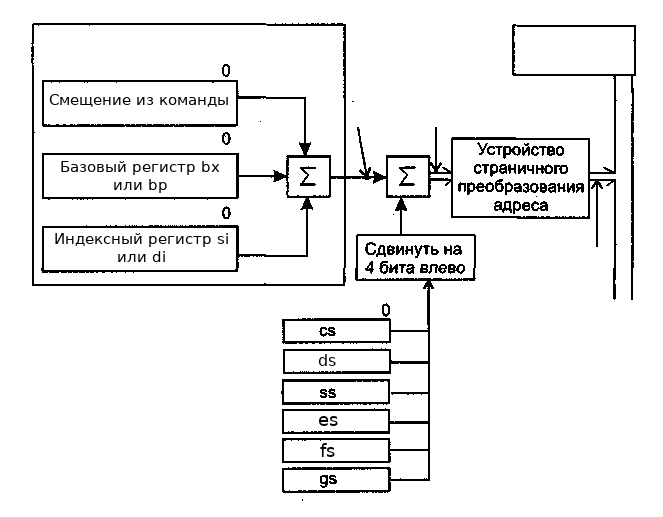
\includegraphics[width=150mm]{pic/physical_address}
  \caption{Механизм формирования физического адреса в реальном режиме}\label{fig:physical_address}
\end{figure}

Исходя из разрядности сегментных регистров, можно утверждать,
что сегментная составляющая адреса (или база сегмента) представляет собой всего
лишь 16-разрядное значение, помещенное в один из сегментных регистров.
Максимальное значение, которое при этом получается, соответствует $ 2^{16} - 1 $.
Если так рассуждать, то получается, что адрес начала сегмента может быть
только в диапазоне 0-64 Кбайт от начала оперативной памяти. Возникает вопрос,
как адресовать остальную часть оперативной памяти вплоть до одного мегабайта с учетом
того, что размер самого сегмента не превышает 64 Кбайт. Дело в том, что в сегмент
ном регистре содержатся только старшие 16 битов физического адреса начала сегмента.
Недостающие младшие четыре бита 20-разрядного адреса получаются сдвигом значения в
сегментном регистре влево на четыре разряда. Эта операция сдвига
выполняется аппаратно и для программного обеспечения абсолютно прозрачна.
Получившееся 20-разрядное значение и является настоящим физическим адресом,
соответствующим началу сегмента. Что касается второго компонента (смещения),
участвующего в образовании физического адреса некоторого объекта в памяти,
то он представляет собой 16-разрядное значение. Это значение может
содержаться явно в команде либо косвенно в одном из регистров общего назначения.
В процессоре эти две составляющие складываются на аппаратном уровне,
в результате получается физический адрес памяти размерностью 20 битов.
Данный механизм образования физического адреса позволяет сделать программное
обеспечение перемещаемым, то есть не зависящим от конкретных адресов
загрузки его в оперативной памяти.

Используя полученные сведения, был изменен исходный код предложенной программы,
как показано на рисунке~\ref{lst:changes}.

\begin{lstlisting}[caption=Модификация исходного кода,label=lst:changes]
.data
    Message db 'Hello world!', CR, LF, EOS
.code
begin:
    ...
    mov dx, 00h ; offset Message
    ...
end begin
\end{lstlisting}

Смещение \textit{Message} относительно начала сегмента данных равно нулю,
следовательно, мы можем подставить это нулевое смещение в исходный код
без риска нарушить работоспособность программы.

Исходный текст разработанной программы находится в приложении~А.